\documentclass[twoside,11pt]{article}

\usepackage{jmlr/jmlr2e}
\usepackage{tikz}
\usetikzlibrary{shapes.geometric, arrows.meta, positioning, calc, shadows}
\usepackage{xcolor}
\usepackage{amssymb}
\usepackage{booktabs}
\usepackage{graphicx}
\usepackage{lastpage}
\usepackage{url}
\usepackage{listings}
\usepackage[most]{tcolorbox}
\tcbuselibrary{listings}
% --- Colors (VS Code–inspired) ---
\definecolor{kwblue}{RGB}{0,0,180}
\definecolor{builtin}{RGB}{0,112,32}
\definecolor{strcolor}{RGB}{186,33,33}
\definecolor{comment}{RGB}{96,128,96}
\definecolor{classcolor}{RGB}{30,120,140}
\definecolor{numcolor}{RGB}{64,128,128}
\definecolor{codebg}{RGB}{249,249,249}
\definecolor{codeframe}{RGB}{200,200,200}
% --- Listings style ---
\lstdefinestyle{python}{
  language=Python,
  basicstyle=\small\ttfamily,
  keywordstyle=\color{kwblue}\bfseries,
  keywordstyle=[2]\color{builtin},
  keywordstyle=[3]\color{classcolor}\bfseries,
  stringstyle=\color{strcolor},
  commentstyle=\color{comment}\itshape,
  numberstyle=\tiny\color{numcolor},
  showstringspaces=false,
  breaklines=true,
  columns=fullflexible,
  keepspaces=true,
  numbers=left,
  numbersep=6pt,
  morekeywords={as,with,True,False,None,self},
  morekeywords=[2]{print,len,range,dict,list,int,float,mean,argsort},
  morekeywords=[3]{ResultWriter,GraFlag,MetricCalculator},
  literate=
    {=}{{{\color{kwblue}=}}}1
    {-}{{{\color{kwblue}-}}}1
    {+}{{{\color{kwblue}+}}}1
    {*}{{{\color{kwblue}*}}}1
}
% --- tcolorbox code blocks ---
\newtcblisting{pycode}{
  listing only,
  listing options={style=python},
  colback=codebg,
  colframe=codeframe,
  boxrule=0.4pt,
  arc=2pt,
  left=2pt, right=2pt, top=1pt, bottom=1pt,
}
\newtcblisting{codebox}{
  listing only,
  listing options={basicstyle=\small\ttfamily,breaklines=true,columns=fullflexible,keepspaces=true},
  colback=codebg,
  colframe=codeframe,
  boxrule=0.4pt,
  arc=2pt,
  left=2pt, right=2pt, top=1pt, bottom=1pt,
}
\usepackage{enumitem}

\jmlrheading{27}{2026}{1-\pageref{LastPage}}{4/26}{}{26-0000}{Ahmed Youcef Benhalima, Seif-Eddine Benkabou, Amin Mesmoudi and Allel Hadjali}

\ShortHeadings{GraFlag: Distributed Benchmarking for Graph Anomaly Detection}{Benhalima, Benkabou, Mesmoudi and Hadjali}
\firstpageno{1}

\begin{document}

\title{GraFlag: Reproducible Distributed Benchmarking\\for Graph Anomaly Detection}

\author{\name Ahmed Youcef Benhalima \email ahmed-youcef.benhalima@ensma.fr \\
       \addr LIAS -- ISAE-ENSMA, Poitiers, France
       \AND
       \name Seif-Eddine Benkabou \email seif.eddine.benkabou@univ-poitiers.fr \\
       \addr LIAS -- Universit\'{e} de Poitiers, France
       \AND
       \name Amin Mesmoudi \email amin.mesmoudi@univ-poitiers.fr \\
       \addr LIAS -- Universit\'{e} de Poitiers, France
       \AND
       \name Allel Hadjali \email allel.hadjali@ensma.fr \\
       \addr LIAS -- ISAE-ENSMA, Poitiers, France}

\editor{TBD}

\maketitle

\begin{abstract}%
GraFlag is an open-source Python framework for \emph{reproducible} benchmarking of graph anomaly detection (GAD) methods on distributed infrastructure. Although libraries like PyGOD provide algorithms and benchmarks like BOND define protocols, no integrated platform combines containerized execution, standardized results, and automated evaluation across distributed GPU clusters---leaving reproducibility fragile. GraFlag closes this gap with a modular architecture on Docker Swarm with NFS-based shared storage and on-demand dataset fetching from original sources via versioned per-dataset metadata, so every experiment replays from a single command on a clean checkout. Nine standardized result types make outputs directly comparable across methods and re-runs, covering static and dynamic graphs at node, edge, and graph granularity. A CLI and web dashboard expose experiment management, real-time monitoring, and automatic generation of metrics and publication-ready plots. Available at \url{https://gbay7.github.io/graflag/}; installable via \texttt{pip install graflag}.
\end{abstract}

\begin{keywords}
  Graph Anomaly Detection, Distributed Benchmarking, Docker Swarm, Reproducibility, Graph Neural Networks
\end{keywords}

\section{Introduction}

Graph anomaly detection (GAD) aims to identify unusual patterns in graph-structured data, with applications in fraud detection, network security, social network analysis, and biological networks~\citep{ma2021comprehensive}. The field has seen rapid growth, with methods spanning diverse paradigms including autoencoders~\citep{ding2019dominant,fan2020anomalydae}, contrastive learning~\citep{xu2022conad,liu2021cola}, generative adversarial networks~\citep{chen2020gaan}, and temporal approaches for dynamic graphs~\citep{liu2023taddy,zheng2019addgraph}.

Several tools have been developed to support GAD research. PyGOD~\citep{liu2024pygod} provides a Python library of detection algorithms with a unified API, while BOND~\citep{liu2022bond} and GADBench~\citep{tang2023gadbench} define standardized evaluation protocols for unsupervised and supervised settings, respectively. In the related domain of time series anomaly detection, TimeEval~\citep{wenig2022timeeval} demonstrates the value of distributed benchmarking toolkits. For tabular data, PyOD~\citep{zhao2019pyod} has become a widely adopted library. However, none of these tools provide an integrated platform that combines containerized execution environments, distributed GPU scheduling, standardized result formats across different graph types, and automated evaluation with visualization, leaving reproducibility of reported GAD benchmarks dependent on ad-hoc scripts, manual dataset downloads, and unpinned local environments.

To bridge this gap, we present GraFlag (\textbf{Gra}ph Anomaly \textbf{Flag}), a distributed benchmarking framework designed for end-to-end reproducibility, with four contributions: (\emph{i})~containerized execution via Docker Swarm with automatic GPU allocation across a multi-node cluster, guaranteeing identical runtime environments across machines and re-runs; (\emph{ii})~nine standardized result types covering three granularities (node, edge, graph) across three temporal modes (static, temporal, streaming), so any reported experiment can be replayed and compared from a single authoritative artifact; (\emph{iii})~a plugin-based evaluation system that computes standard metrics and generates publication-ready visualizations directly from that artifact; and (\emph{iv})~a CLI and web dashboard with real-time experiment monitoring, complemented by on-demand dataset fetching from original sources via versioned per-dataset metadata.

\section{Framework Design and Implementation}

GraFlag is a lightweight Python client (Python~3.10+, depending only on \texttt{docker}, \texttt{pyyaml}, \texttt{flask}, and \texttt{flask-socketio}) that orchestrates experiments on a remote GPU cluster. The client itself needs no GPU; all computation is offloaded.

\textbf{Architecture.} The framework adopts a three-layer architecture (Figure~\ref{fig:arch}). The \emph{Client Layer} provides the CLI, Python API, and web dashboard, communicating with the cluster via SSH tunnels. The \emph{Cluster Layer} is a Docker Swarm comprising a manager node with a local image registry and GPU-enabled worker nodes. The \emph{Shared Storage Layer} is an NFS-mounted directory organized into \texttt{methods/}, \texttt{datasets/}, and \texttt{experiments/} repositories, accessible from all nodes.

\begin{figure*}[t]
   \centering
   \resizebox{0.78\textwidth}{!}{% --- Named Color Definitions ---
\definecolor{clientBorder}{RGB}{70,110,180}
\definecolor{clientBg}{RGB}{232,240,254}
\definecolor{clientLabel}{RGB}{50,85,150}
\definecolor{clusterBorder}{RGB}{50,140,110}
\definecolor{clusterBg}{RGB}{232,248,240}
\definecolor{clusterLabel}{RGB}{30,110,85}
\definecolor{storageBorder}{RGB}{200,140,60}
\definecolor{storageBg}{RGB}{255,243,228}
\definecolor{storageLabel}{RGB}{160,110,30}
\definecolor{workflowBorder}{RGB}{120,100,160}
\definecolor{workflowBg}{RGB}{245,243,248}
\definecolor{workflowLabel}{RGB}{90,75,130}
%
\begin{tikzpicture}[
    font=\small\sffamily, % Sans-serif for clean scientific look
    node distance=0.5cm and 0.4cm,
    % --- Layer Base ---
    layerBase/.style={rectangle, rounded corners=4pt, thick, line width=0.8pt},
    % --- Component Styles ---
    comp/.style={rectangle, rounded corners=2pt, thick, line width=0.6pt,
        fill=white, draw=clientBorder, minimum width=2.8cm, minimum height=0.9cm, align=center,
        drop shadow={shadow xshift=0.4pt, shadow yshift=-0.4pt, fill=black!8}},
    nodeBox/.style={rectangle, rounded corners=2pt, thick, line width=0.6pt,
        fill=white, draw=clusterBorder, minimum width=3.2cm, minimum height=1.6cm, align=left,
        drop shadow={shadow xshift=0.4pt, shadow yshift=-0.4pt, fill=black!8}},
    storageBox/.style={cylinder, shape border rotate=90, thick, line width=0.6pt,
        fill=white, draw=storageBorder, minimum width=1.2cm, minimum height=1cm,
        drop shadow={shadow xshift=0.4pt, shadow yshift=-0.4pt, fill=black!8}},
    stepBox/.style={rectangle, rounded corners=6pt, line width=0.6pt,
        draw=workflowBorder, fill=workflowBg, minimum width=2.5cm, minimum height=0.6cm},
    % --- Arrow Styles ---
    controlArrow/.style={-{Stealth[scale=0.7]}, color=clientBorder, line width=1pt},
    dataArrow/.style={{Stealth[scale=0.7]}-{Stealth[scale=0.7]}, color=storageBorder, line width=1pt},
    flowArrow/.style={-{Stealth[scale=0.6]}, color=workflowBorder, line width=0.9pt},
    connLine/.style={color=clientBorder, line width=0.7pt, dash pattern=on 3pt off 1.5pt}
]

    % --- 1. CLIENT LAYER ---
    \node[layerBase, fill=clientBg, draw=clientBorder, minimum width=13.5cm, minimum height=1.7cm] (CL) at (6.5, 0) {};
    \node[anchor=north west, font=\footnotesize\bfseries\sffamily, text=clientLabel, xshift=5pt, yshift=-3pt] at (CL.north west) {Client Layer \textnormal{\footnotesize(Local Machine)}};

    \node[comp] (cli)  at (1.5, -0.2)  {\textbf{CLI\,/\,API} \\ \scriptsize\color{black!60} User Interface};
    \node[comp] (core) at (4.8, -0.2)  {\textbf{Core} \\ \scriptsize\color{black!60} Orchestration};
    \node[comp] (ssh)  at (8.1, -0.2)  {\textbf{SSH} \\ \scriptsize\color{black!60} Secure Transport};
    \node[comp] (dock) at (11.4, -0.2) {\textbf{Docker} \\ \scriptsize\color{black!60} Swarm Control};

    \draw[connLine] (cli) -- (core) -- (ssh) -- (dock);

    % --- 2. CLUSTER LAYER ---
    \node[layerBase, fill=clusterBg, draw=clusterBorder, minimum width=13.5cm, minimum height=2.4cm, below=0.6cm of CL] (CLL) {};
    \node[anchor=north west, font=\footnotesize\bfseries\sffamily, text=clusterLabel, xshift=5pt, yshift=-3pt] at (CLL.north west) {Cluster Layer \textnormal{\footnotesize(Docker Swarm)}};

    \node[nodeBox] (manager) at (2.1, -2.9) {\textbf{\scriptsize Manager Node} \\ \tiny\color{black!65} $\bullet$~Swarm Orchestration \\ \tiny\color{black!65} $\bullet$~Local Registry \\ \tiny\color{black!65} $\bullet$~NFS Server};
    \node[nodeBox] (worker)  at (6.5, -2.9) {\textbf{\scriptsize Worker Nodes} \\ \tiny\color{black!65} $\bullet$~GPU Acceleration \\ \tiny\color{black!65} $\bullet$~Method Execution \\ \tiny\color{black!65} $\bullet$~NFS Clients};
    \node[nodeBox, dashed] (services) at (10.9, -2.9) {\textbf{\scriptsize Dynamic Services} \\ \tiny\color{black!65} $\bullet$~Runtime Containers \\ \tiny\color{black!65} $\bullet$~Resource Isolation \\ \tiny\color{black!65} $\bullet$~Sidecar Monitoring};

    % --- 3. STORAGE LAYER ---
    \node[layerBase, fill=storageBg, draw=storageBorder, minimum width=13.5cm, minimum height=1.8cm, below=0.6cm of CLL] (SL) {};
    \node[anchor=north west, font=\footnotesize\bfseries\sffamily, text=storageLabel, xshift=5pt, yshift=-3pt] at (SL.north west) {Shared Storage \textnormal{\footnotesize(NFS)}};

    \node[storageBox] (d1) at (2, -5.7) {};   \node[below=-0.5 of d1, font=\tiny\bfseries\ttfamily, text=storageLabel] {datasets/};
    \node[storageBox] (d2) at (5, -5.7) {};   \node[below=-0.5 of d2, font=\tiny\bfseries\ttfamily, text=storageLabel] {methods/};
    \node[storageBox] (d3) at (8, -5.7) {};   \node[below=-0.5 of d3, font=\tiny\bfseries\ttfamily, text=storageLabel] {experiments/};
    \node[storageBox] (d4) at (11, -5.7) {};  \node[below=-0.5 of d4, font=\tiny\bfseries\ttfamily, text=storageLabel] {libs/};

    % --- 4. LOGICAL WORKFLOW ---
    \node[anchor=west, font=\scriptsize\bfseries\sffamily, text=workflowLabel] (wfLabel) at (0, -6.8) {Logical Workflow:};
    \node[stepBox] (s0) at (1.5, -7.5) {\scriptsize\texttt{0.\;setup}};
    \node[stepBox] (s1) at (4.8, -7.5) {\scriptsize\texttt{1.\;benchmark}};
    \node[stepBox] (s2) at (8.1, -7.5) {\scriptsize\texttt{2.\;logs}};
    \node[stepBox] (s3) at (11.4, -7.5) {\scriptsize\texttt{3.\;evaluate}};

    \draw[flowArrow] (s0) -- (s1);
    \draw[flowArrow] (s1) -- (s2);
    \draw[flowArrow] (s2) -- (s3);

    % --- INTER-LAYER CONNECTORS ---
    \draw[controlArrow] (CL.south) -- (CLL.north) node[midway, right, font=\tiny\sffamily, text=clientLabel] {Control (SSH)};
    \draw[dataArrow] (CLL.south) -- (SL.north) node[midway, right, font=\tiny\sffamily, text=storageLabel] {Data (NFS)};

\end{tikzpicture}}
   \caption{GraFlag architecture. The client orchestrates experiments remotely via SSH. Docker Swarm schedules method containers on GPU-enabled workers. All data flows through NFS-mounted shared storage.}
   \label{fig:arch}
\end{figure*}

\begin{table}[t]
\centering
\caption{Detection methods in GraFlag. PyGOD methods~\citep{liu2024pygod} are integrated via \texttt{graflag\_bond}; custom methods use \texttt{ResultWriter}. Additional methods are continuously being integrated.}
\label{tab:methods}
\footnotesize
\begin{tabular}{@{}lllll@{}}
\toprule
\textbf{Method} & \textbf{Graph} & \textbf{Backbone} & \textbf{GPU} & \textbf{Reference} \\
\midrule
\emph{PyGOD methods} & Static & Various & Yes/No & \citet{liu2024pygod} \\
\multicolumn{5}{@{}l@{}}{\scriptsize\quad (DOMINANT, CONAD, AnomalyDAE, CoLA, GAAN, GAE, SCAN, etc.)} \\
\midrule
TADDY      & Dynamic    & Transformer & Yes & \citet{liu2023taddy} \\
AddGraph   & Dynamic    & GCN         & Yes & \citet{zheng2019addgraph} \\
DynWalk    & Dynamic    & Embedding   & No  & \citet{yu2018netwalk} \\
StrGNN     & Dynamic    & GNN         & Yes & \citet{cai2021strgnn} \\
GeneralDyG & Dynamic    & GNN         & Yes & \citet{yang2025generaldyg} \\
GADY       & Dynamic    & GNN         & Yes & \citet{lou2023gady} \\
SLADE      & Dynamic    & GNN         & Yes & \citet{lee2024slade} \\
AnoGraph   & Dynamic    & Sketch      & No  & \citet{bhatia2023anograph} \\
StreamSpot & Dynamic    & Sketch      & No  & \citet{manzoor2016streamspot} \\
\bottomrule
\end{tabular}
\end{table}

\textbf{Method Integration.} To run on this infrastructure, each detection method is packaged as a Docker image. GraFlag provides two integration patterns. For methods available in the PyGOD library~\citep{liu2024pygod}, the \texttt{graflag\_bond} adapter handles data loading, training, and result writing---requiring only a \texttt{.env} configuration and a \texttt{Dockerfile}. For other methods, a custom script uses the \texttt{ResultWriter} API to produce standardized outputs (Code~Demo~1). Table~\ref{tab:methods} lists the currently integrated methods.

\begin{figure}[!ht]
\small\textbf{Code Demo 1:} Integrating a custom detection method.
\begin{pycode}
from graflag_runner import ResultWriter
writer = ResultWriter()
writer.spot("training", epoch=e, loss=l)
writer.save_scores(
    result_type="EDGE_STREAM_ANOMALY_SCORES",
    scores=scores, ground_truth=ground_truth)
writer.finalize()
\end{pycode}
\end{figure}

\textbf{Standardized Result Types.} Regardless of the integration pattern, every method must produce results in one of nine standardized formats, defined as the Cartesian product of three granularities---node, edge, and graph---and three temporal modes: \emph{static} (1D score vectors), \emph{temporal} (2D matrices indexed by entities~$\times$~timestamps), and \emph{streaming} (sparse 1D scores over a continuous timeline). The same nine-way classification drives the evaluator's metric dispatch.

\textbf{Evaluation.} Once an experiment completes, the \texttt{graflag\_evaluator} computes AUC-ROC, AUC-PR, F1@K, Precision@K, and Recall@K from the standardized results, and generates publication-ready plots. Custom metrics can be added via a plugin system: \texttt{register\_metric()} extracts the function source and persists it as a plugin file on the shared storage, so that the containerized evaluator loads it at runtime (Code~Demo~2).

\begin{figure}[!ht]
\small\textbf{Code Demo 2:} Programmatic batch benchmarking via the Python API.
\begin{pycode}
from graflag import GraFlag
# Register a custom metric (persisted as plugin file)
def hits_at_100(scores, ground_truth, **kw):
    top = scores.argsort()[-100:]
    return {"hits@100": ground_truth[top].mean()}
gf = GraFlag()
gf.register_metric("EDGE_STREAM_ANOMALY_SCORES", hits_at_100)
# Run all method/dataset combinations
for m in gf.list_methods():
    for d in gf.list_datasets():
        exp = gf.run(m.name, d.name, build=True)
        gf.evaluate(exp)
        res = gf.get_evaluation_results(exp)
        print(f"{m.name}/{d.name}: AUC={res.metrics['auc_roc']:.3f}")
\end{pycode}
\end{figure}

\textbf{Workflow, Interfaces, and Reproducibility.} The entire pipeline---from cluster setup through execution to evaluation---is exposed via a CLI (\texttt{graflag setup}, \texttt{graflag run}, \texttt{graflag evaluate}), the Python API shown above, and a web dashboard (\texttt{graflag gui}) with live status badges, log streaming, and one-click evaluation. Every experiment persists its full configuration, so any past run replays with \texttt{graflag run -{}-from-config}.

\section{Quality and Accessibility}

GraFlag is released under the MIT license and installable via \texttt{pip install graflag}. It includes a virtual development cluster (\texttt{graflag devcluster}) for local testing without physical infrastructure.

\section{Conclusion and Future Plans}
\vspace{-2pt}
GraFlag provides containerized execution, standardized results, and automated evaluation for graph anomaly detection on Docker Swarm. Future work includes Apptainer/Singularity for HPC, statistical comparison tools, and hyperparameter tuning.
\vspace{-4pt}
\acks{LIAS laboratory, ISAE-ENSMA / Universit\'{e} de Poitiers.}

\vskip 0.2in
\bibliography{graflag}

\newpage
\appendix

\section{Comparison with Related Tools}
\label{app:comparison}

Table~\ref{tab:comparison} compares GraFlag with existing tools for graph anomaly detection and related domains. PyGOD~\citep{liu2024pygod} is a Python library of detection algorithms with a unified API; its repository also includes the BOND~\citep{liu2022bond} benchmark evaluation code. GADBench~\citep{tang2023gadbench} evaluates supervised and unsupervised methods on static graphs. None of these tools offer distributed execution or containerized environments. TimeEval~\citep{wenig2022timeeval} demonstrates the value of containerized, distributed benchmarking for time series but does not support graph data. PyOD~\citep{zhao2019pyod} targets tabular outlier detection. GraFlag is the first tool to integrate all of these capabilities for graph anomaly detection.

\begin{table}[h]
\centering
\caption{Feature comparison of GraFlag with related tools. \checkmark\ = supported, $\times$ = not supported, $\circ$ = partial.}
\label{tab:comparison}
% \footnotesize
\setlength{\tabcolsep}{3pt}
\begin{tabular}{@{}lccccc@{}}
\toprule
\textbf{Feature} & \textbf{GraFlag} & \textbf{PyGOD} & \textbf{GADBench} & \textbf{TimeEval} & \textbf{PyOD} \\
\midrule
Data domain        & Graph    & Graph  & Graph  & Time series & Tabular \\
Dynamic graphs     & \checkmark & $\times$ & $\times$ & --- & --- \\
Distributed exec.  & \checkmark & $\times$ & $\times$ & \checkmark & $\times$ \\
Containerized      & \checkmark & $\times$ & $\times$ & \checkmark & $\times$ \\
GPU scheduling     & \checkmark & $\times$ & $\times$ & $\times$ & $\times$ \\
% Std.\ result types & 9        & 1      & 1      & 1 & 1 \\
Auto.\ evaluation  & \checkmark & $\circ$ & \checkmark & \checkmark & $\circ$ \\
Web dashboard      & \checkmark & $\times$ & $\times$ & $\circ$ & $\times$ \\
Config replay      & \checkmark & $\times$ & $\times$ & $\times$ & $\times$ \\
Plugin metrics     & \checkmark & $\times$ & $\times$ & $\times$ & $\times$ \\
\bottomrule
\end{tabular}
\end{table}
% GPU scheduling: Automatic assignment of containers to GPU-enabled worker nodes via Docker Swarm's generic resource scheduler, as opposed to simply using a locally available GPU.
Key differentiators include: (\emph{i})~GraFlag is the only graph-focused tool with distributed, containerized execution; (\emph{ii})~nine standardized result types cover three granularities across three temporal modes, while other tools support only node-level scores; (\emph{iii})~the plugin-based metric system allows domain-specific evaluation without modifying framework code; and (\emph{iv})~configuration replay via \texttt{service\_config.json} enables exact reproduction of any past experiment.

\section{Shared Storage and Project Structure}
\label{app:structure}

GraFlag separates the orchestration package from the shared data layer. The main \texttt{graflag} package (installed via pip) contains the CLI, Python API, web dashboard, and virtual development cluster. The NFS-mounted shared storage holds all methods, datasets, experiment results, and shared libraries accessible to every cluster node.

\textbf{Main Package Structure.}
\begin{codebox}
graflag/
|-- cli.py           # CLI (argparse)
|-- core.py          # GraFlag orchestration class
|-- config.py        # Configuration management
|-- models.py        # Dataclasses (MethodInfo, etc.)
|-- ssh.py           # SSH/rsync operations
|-- docker_ops.py    # Docker Swarm operations
|-- api.py           # Python API (for GUI)
|-- gui/             # Flask web dashboard
`-- devcluster/      # Virtual cluster (Docker Compose)
\end{codebox}

\textbf{NFS Shared Storage Layout.}
\begin{codebox}
/shared/                          # NFS mount point
|-- methods/                      # Detection methods
|   `-- <method_name>/
|       |-- .env                  # Metadata + parameters
|       |-- Dockerfile
|       `-- [train_graflag.py]    # Custom methods only
|-- datasets/
|   `-- <dataset_name>/           # Graph data files
|-- experiments/
|   `-- exp__<method>__<dataset>__<timestamp>/
|       |-- results.json          # Scores + ground truth
|       |-- service_config.json   # Reproducible config
|       |-- service_details.json  # Docker service info
|       |-- training.csv          # Training curves
|       `-- eval/                 # Evaluation outputs
|           |-- evaluation.json
|           |-- roc_curve.png
|           |-- pr_curve.png
|           `-- score_distribution.png
`-- libs/
    |-- graflag_runner/           # Execution framework
    |-- graflag_bond/             # PyGOD adapter
    `-- graflag_evaluator/        # Evaluation framework
\end{codebox}

\section{Method Integration Guide}
\label{app:integration}

GraFlag supports two integration patterns. This section provides complete examples for each.

\subsection{Pattern A: Custom Methods}

For a custom method, two files are needed: a \texttt{.env} configuration, a \texttt{Dockerfile}, and require an entry point \texttt{COMMAND} which is specified by the \texttt{.env} configuration. Defining a new method, needs usually three steps:

\textbf{Step 1: Method configuration (\texttt{.env}).} The \texttt{.env} file defines method metadata and default parameters. Parameters prefixed with an underscore are injected as environment variables into the container. When the container entry point uses the \texttt{-{}-pass-env-args} flag, these variables are converted to command-line arguments (e.g., \texttt{\_MAX\_EPOCH=200} becomes \texttt{-{}-max\_epoch~200}). The \texttt{COMMAND} field specifies the executable invoked inside the container.

The optional \texttt{SUPPORTED\_DATASETS} field lists comma-separated patterns used to filter compatible datasets; wildcards are expanded to regular expressions (e.g., \texttt{bond\_*} matches \texttt{bond\_.*}).

\begin{codebox}
METHOD_NAME=taddy
DESCRIPTION=Temporal Anomaly Detection via Transformer
SOURCE_CODE=https://github.com/yixingwang0517/TADDY_pytorch
SUPPORTED_DATASETS=uci,btc_alpha,btc_otc,digg
COMMAND=python3 train_graflag.py

# Default parameters (injected as env vars)
_MAX_EPOCH=200
_LEARNING_RATE=0.001
_EMBEDDING_DIM=32
_NUM_HIDDEN_LAYERS=2
_NUM_ATTENTION_HEADS=2
_WINDOW_SIZE=2
_GPU=0
\end{codebox}

\textbf{Step 2: Container definition (\texttt{Dockerfile}).}

\begin{codebox}
FROM nvidia/cuda:12.1.0-runtime-ubuntu22.04
RUN apt-get update && apt-get install -y python3 python3-pip git
RUN git clone <source_repo> /app/src
COPY train_graflag.py /app/
RUN pip install ./libs/graflag_runner torch torch-geometric
WORKDIR /app
CMD ["python3", "-m", "graflag_runner", "--pass-env-args"]
\end{codebox}

The \texttt{graflag\_runner} module serves as the container entry point. It reads \texttt{COMMAND} from the environment, monitors resource usage (CPU, memory, GPU), executes the command, and captures output. Shared libraries (\texttt{graflag\_runner}, \texttt{graflag\_bond}) are installed inside the container via the Dockerfile, since the build context is the entire shared storage directory.

\textbf{Step 3: Integration script.} The script referenced by \texttt{COMMAND} uses the \texttt{ResultWriter} API to produce standardized outputs. Since \texttt{graflag\_runner} is installed inside the container (Step~2), it can be imported directly:

\begin{pycode}
import os, argparse
from graflag_runner import ResultWriter

parser = argparse.ArgumentParser()
parser.add_argument("--max_epoch", type=int)
parser.add_argument("--learning_rate", type=float)
# ... additional parameters
args = parser.parse_args()

writer = ResultWriter()  # reads EXP env var

# Load data from $DATA env var
data = load_data(os.environ["DATA"])

# Training loop
for epoch in range(args.max_epoch):
    loss = train_step(model, data)
    writer.spot("training", epoch=epoch, loss=loss)

# Save standardized results
scores = model.predict(data)
writer.save_scores(
    result_type="EDGE_STREAM_ANOMALY_SCORES",
    scores=scores,
    ground_truth=data.labels)
writer.add_resource_metrics(
    exec_time_ms=elapsed, peak_memory_mb=mem)
writer.finalize()
\end{pycode}

\subsection{Pattern B: PyGOD via graflag\_bond}

For methods available in the PyGOD library~\citep{liu2024pygod}, only a \texttt{.env} and a \texttt{Dockerfile} are needed. The \texttt{graflag\_bond} adapter handles data loading, model instantiation, training, and result writing automatically.

\begin{codebox}
# .env for bond_dominant
METHOD_NAME=bond_dominant
DESCRIPTION=Deep Anomaly Detection on Attributed Networks
SUPPORTED_DATASETS=bond_*
COMMAND=python3 -m graflag_bond.train

_HID_DIM=64
_NUM_LAYERS=4
_DROPOUT=0
_LR=0.004
_EPOCH=100
_CONTAMINATION=0.1
\end{codebox}

The \texttt{graflag\_bond.train} module dynamically resolves the detector class from the method name (e.g., \texttt{bond\_dominant} $\rightarrow$ \texttt{pygod.detector.Dominant}), extracts all \texttt{\_}-prefixed environment variables, performs type conversion using the detector's constructor signature, trains the model, and saves \texttt{NODE\_ANOMALY\_SCORES} via \texttt{ResultWriter}.

\textbf{Parameter Override at Runtime.} Users can override any default parameter without modifying the \texttt{.env} file:
\begin{codebox}
graflag run -m bond_dominant -d bond_inj_cora \
    --params EPOCH=200 LR=0.001 HID_DIM=128
\end{codebox}

\section{Supported Datasets}
\label{app:datasets}

GraFlag currently includes 34 benchmark datasets organized into two categories, as shown in Table~\ref{tab:datasets}. Static datasets (14) are sourced from the BOND benchmark~\citep{liu2022bond} and comprise six synthetically generated graphs, five real-world networks, and three networks with injected anomalies. Dynamic datasets (20) cover financial transaction networks, communication networks, and social networks, with various temporal representations (snapshots, continuous edge streams).

\begin{table}[h]
\centering
\caption{Benchmark datasets in GraFlag. Datasets are organized by graph type (static vs.\ dynamic) and data source. Additional datasets can be added by placing graph files in the shared \texttt{datasets/} directory.}
\label{tab:datasets}
\footnotesize
\setlength{\tabcolsep}{4pt}
\begin{tabular}{@{}llp{5.2cm}@{}}
\toprule
\textbf{Category} & \textbf{Count} & \textbf{Datasets} \\
\midrule
\multicolumn{3}{@{}l}{\emph{Static Graphs}} \\
\quad BOND synthetic & 6 & bond\_gen\_\{100, 500, 1K, 5K, 10K, time\} \\
\quad BOND injected  & 3 & bond\_inj\_\{amazon, cora, flickr\} \\
\quad BOND real-world & 5 & bond\_\{books, disney, enron, reddit, weibo\} \\
\midrule
\multicolumn{3}{@{}l}{\emph{Dynamic Graphs}} \\
\quad Financial       & 6 & btc\_alpha(\_snapshot), btc\_otc(\_snapshot), generaldyg\_btc\_\{alpha, otc\} \\
\quad Communication   & 5 & uci(\_snapshot), email\_snapshot(\_005), gady\_email\_dnc \\
\quad Social          & 1 & digg \\
\quad Intrusion       & 2 & anograph\_\{darpa, iscx\} \\
\quad Streaming       & 6 & slade\_\{bitcoinalpha, bitcoinotc, hijack, wikipedia, new\}, streamspot\_all \\
\bottomrule
\end{tabular}
\end{table}

\section{Evaluation System}
\label{app:evaluation}

\subsection{Computed Metrics}

The \texttt{graflag\_evaluator} computes the following metrics for all nine result types. %For temporal and streaming types, scores are flattened across time steps before metric computation, with support for ragged arrays (snapshots with varying numbers of entities).

\begin{itemize}[nosep,leftmargin=*]
\item \textbf{AUC-ROC}: Area under the Receiver Operating Characteristic curve, measuring discrimination ability across all thresholds.
\item \textbf{AUC-PR}: Area under the Precision-Recall curve, more informative than AUC-ROC under class imbalance.
\item \textbf{Precision@K}, \textbf{Recall@K}, \textbf{F1@K}: Precision, recall, and F1 score when predicting the top $K$ scored entities as anomalies, where $K$ equals the true number of anomalies.
\item \textbf{Best F1}: Maximum F1 score across all decision thresholds with the corresponding threshold value.
\end{itemize}

Additional type-specific metrics are computed: temporal span and timestamp count for temporal/streaming types; unique edge and node counts for edge-level types.

\subsection{Custom Metric Plugins}

Custom metrics can be registered for any result type via a plugin system. The Python API method \texttt{register\_metric()} extracts the function source and writes it as a plugin file on the cluster. The evaluator loads plugins from two directories:

\begin{itemize}[nosep,leftmargin=*]
\item \textbf{Global}: \texttt{libs/graflag\_evaluator/plugins/} (all evaluations).
\item \textbf{Per-experiment}: \texttt{experiments/<exp>/custom\_metrics/}.
\end{itemize}

Each plugin file imports \texttt{MetricCalculator} and calls \texttt{register\_metric()} at module level. The plugin file resides on NFS-mounted shared storage, so the containerized evaluator can load it at runtime. Plugins can also be created manually.

\subsection{Generated Visualizations}

The evaluator produces three standard plots per experiment, saved as PNG files in the \texttt{eval/} subdirectory:

\begin{itemize}[nosep,leftmargin=*]
\item \textbf{ROC Curve}
\item \textbf{Precision-Recall Curve}
\item \textbf{Score Distribution}
\end{itemize}

Additionally, for each CSV file created by \texttt{ResultWriter.spot()} during training (e.g., \texttt{training.csv}), the evaluator generates training curve plots showing metric evolution over epochs. These plots are visible in the web dashboard (Figure~\ref{fig:dashboard}).

\section{Web Dashboard and Virtual Development Cluster}
\label{app:dashboard}

\subsection{Web Dashboard}

The web dashboard (\texttt{graflag gui}) provides a browser-based interface for experiment management built with Flask and Flask-SocketIO (Figure~\ref{fig:dashboard}). Key features include:

\begin{itemize}[nosep,leftmargin=*]
\item \textbf{Cluster Overview}: Real-time node status, GPU availability, and running services.
\item \textbf{Experiment Management}: Browse methods and datasets, configure and submit experiments, monitor progress with live log streaming via WebSocket.
\item \textbf{One-Click Evaluation}: Trigger evaluation and view metrics and plots directly in the browser.
\item \textbf{Experiment History}: List past experiments with status badges, access results and evaluation outputs.
\end{itemize}

The dashboard communicates with the cluster through the same \texttt{GraFlag} Python API used by the CLI, ensuring consistent behavior. Background threads poll for state changes and push updates to connected clients via WebSocket, avoiding page reloads. All long-running operations (build, run, evaluate) execute in background threads to keep the interface responsive.

\begin{figure}[ht]
\centering
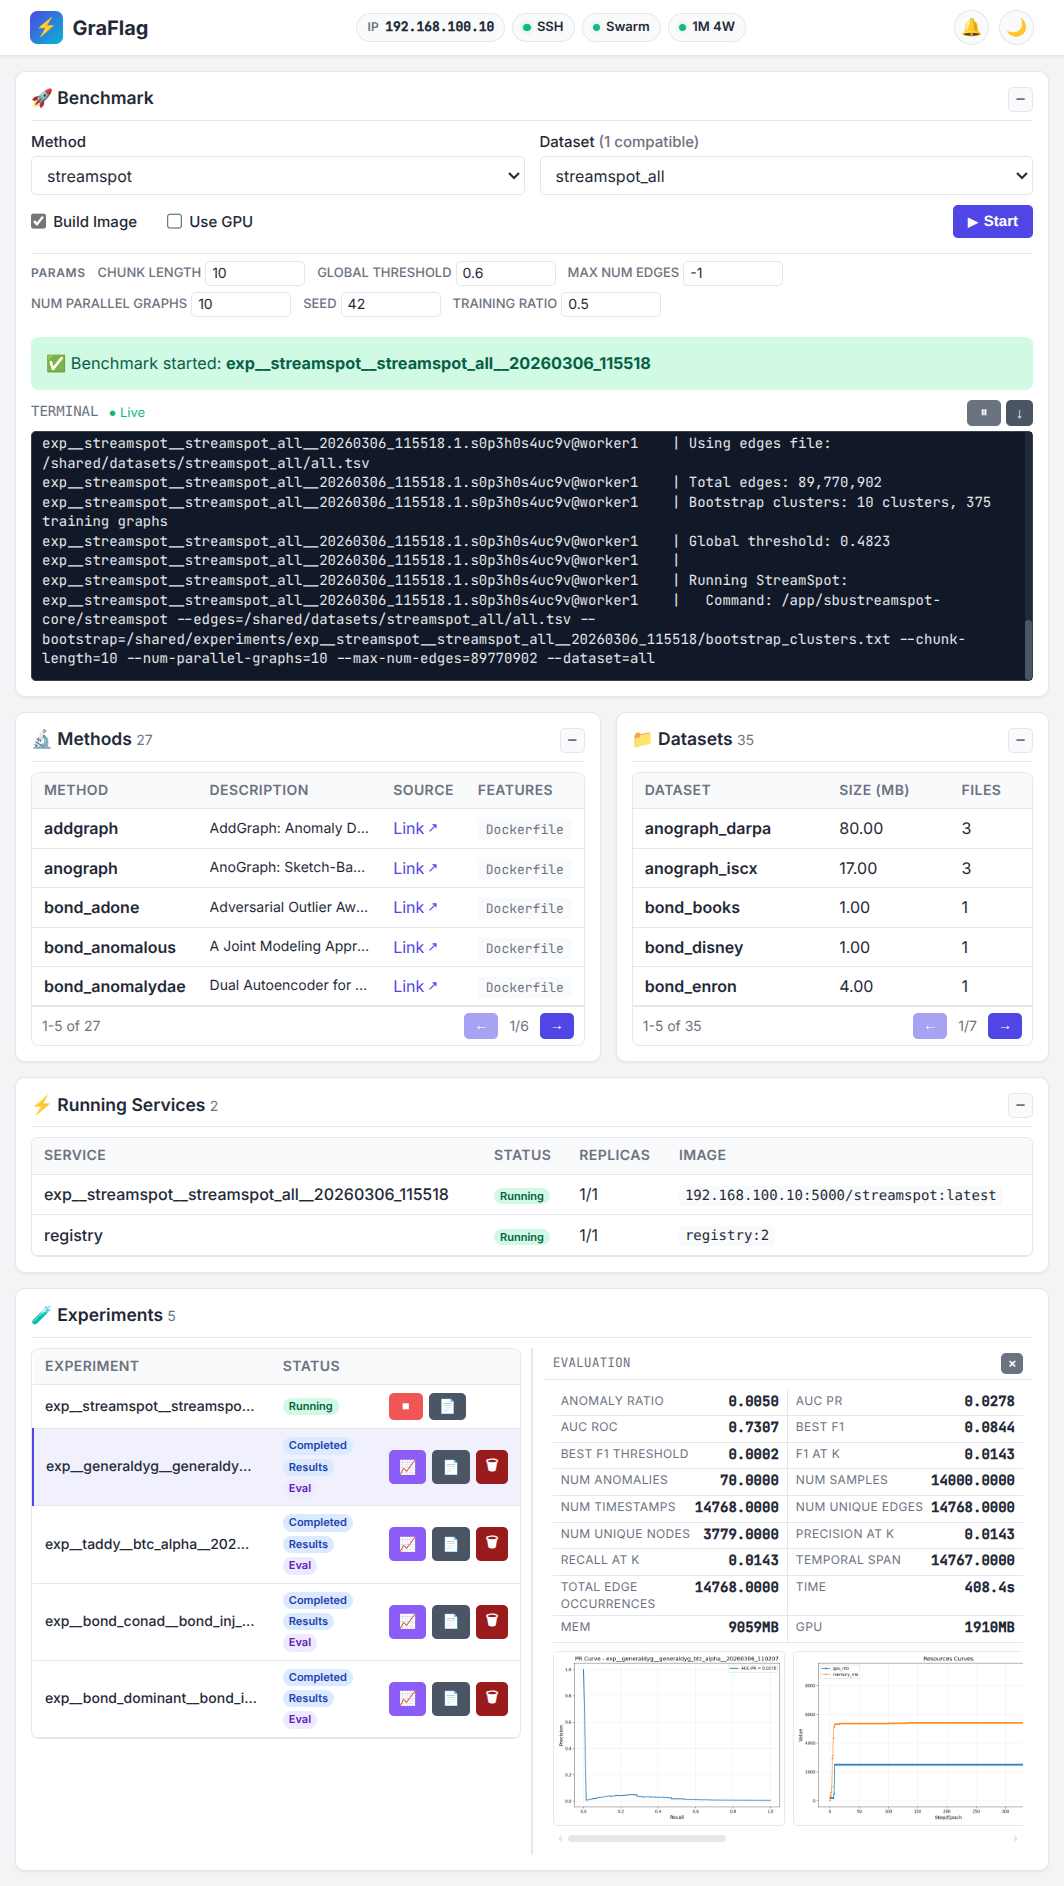
\includegraphics[height=0.67\textheight]{dashboard.png}
\caption{GraFlag web dashboard showing the experiment monitoring interface with real-time log streaming and cluster status.}
\label{fig:dashboard}
\end{figure}

\subsection{Virtual Development Cluster}

GraFlag includes a virtual development cluster (\texttt{graflag devcluster}) that replicates the full distributed environment locally using Docker Compose. This allows users to develop and test methods, debug configurations, and explore the framework without access to physical GPU infrastructure.

The virtual cluster creates Docker-in-Docker containers (one manager and workers) on a custom bridge network with fixed IPs, NFS-based shared storage between containers, and SSH connectivity. It mirrors the production architecture: the manager runs a Docker Swarm, a local registry, and an NFS server, while workers join the swarm and mount the shared directory. The cluster is deployed with a single command:

\begin{codebox}
graflag devcluster --hosts hosts.yml
\end{codebox}

where \texttt{hosts.yml} specifies the network subnet, manager IP, and worker IPs. GPU passthrough is supported when NVIDIA drivers are available on the host. The cluster is torn down with \texttt{graflag devcluster -{}-down}.

\section{CLI Reference}
\label{app:cli}

Table~\ref{tab:cli} lists all GraFlag CLI commands.

\begin{table}[h]
\centering
\caption{GraFlag CLI commands. All commands are invoked as \texttt{graflag <command>}.}
\label{tab:cli}
\footnotesize
\begin{tabular}{@{}lp{6cm}@{}}
\toprule
\textbf{Command} & \textbf{Description} \\
\midrule
\texttt{setup}      & Initialize Docker Swarm on manager and join workers \\
\texttt{run}        & Execute a method on a dataset (\texttt{-m}, \texttt{-d}, \texttt{-{}-build}, \texttt{-{}-params}, \texttt{-{}-from-config}) \\
\texttt{evaluate}   & Compute metrics and generate plots for an experiment (\texttt{-e}) \\
\texttt{list}       & List resources: \texttt{methods}, \texttt{datasets}, \texttt{experiments}, \texttt{services} \\
\texttt{status}     & Show cluster status (nodes, services, shared storage) \\
\texttt{logs}       & View experiment logs (\texttt{-e}, \texttt{-{}-follow}, \texttt{-{}-tee}) \\
\texttt{stop}       & Stop a running experiment (\texttt{-e}, \texttt{-{}-rm}) \\
\texttt{copy}       & Transfer files to/from cluster (\texttt{-{}-from-remote}, \texttt{-r}) \\
\texttt{sync}       & Sync local method or library to remote (\texttt{-{}-lib}) \\
\texttt{gui}        & Start web dashboard (\texttt{-{}-port}, \texttt{-{}-debug}) \\
\texttt{devcluster} & Deploy/teardown virtual cluster (\texttt{-{}-hosts}, \texttt{-{}-down}) \\
\bottomrule
\end{tabular}
\end{table}

\end{document}
